\noindent \textred{10.}
{Randomly cut a line segment $(0,1)$ into three pieces. What is the probability that these three pieces can form a right triangle with at least one side less than 0.25?
\begin{figure}[!h]
    \centering
    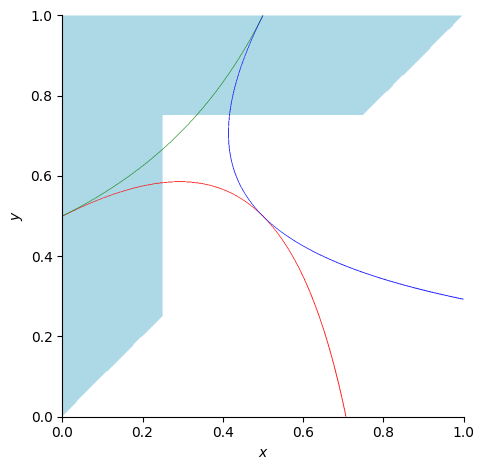
\includegraphics[width=0.5\linewidth]{HWs//HW2//figures/10.png}
\end{figure}

\noindent \myAnswer{
Let $X$ and $Y$ be the random variable that represent the locations of two random breaks, so $X, Y \sim \text{Uniform}(0,1)$. Without losing generality, let's consider the situation that $X < Y$. With the restriction that at least one side is less than 0.25, we can draw the feasible region in the figure above (light blue). \\
To form a right triangle, three sides $X, Y, 1-Y$ must satisfy the Pythagorean theorem:
\begin{align*}
    x^2 + (y-x)^2 = (1-y)^2 &\quad, x + y - x > 1 - y ~(y > 0.5) \\
    x^2 + (1-y)^2 = (y-x)^2 &\quad, x + 1 - y > y - x ~(y - x < 0.5) \\
    (y-x)^2 + (1-y)^2 = x^2 &\quad, x + y - x > 1-y ~(x < 0.5)
\end{align*}
These three cases are plotted in the figure with \textred{red}, \textgreen{green}, and blue lines respectively. \\
Although there are infinite points in the figure satisfying the Pythagorean theorem, there is no area. Therefore, the probability that these three pieces can form a right triangle with at least one side less than 0.25 is \underline{0}.
}